% Important: If latex complains about unicode characters,
% please use "\usepackage[utf8x]{inputenc}" in your preamble
% You can change the size of the picture by putting it into the construct:
% 1) \resizebox{10cm}{!}{"below picture"} to scale horizontally to 10 cm
% 2) \resizebox{!}{15cm}{"below picture"} to scale vertically to 15 cm
% 3) \resizebox{10cm}{15cm}{"below picture"} a combination of above two
% It is not recomended to use the scale option of the tikzpicture environment.
\resizebox{10cm}{!}{
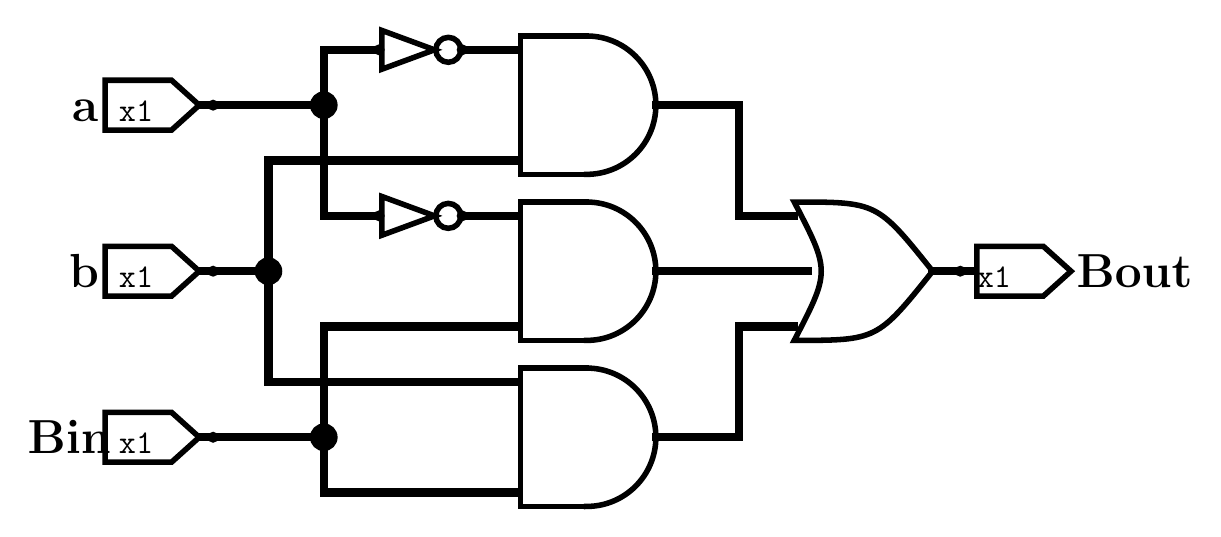
\begin{tikzpicture}[x=1pt,y=-1pt,line cap=rect]
\def\logisimfontA#1{\fontfamily{cmr}{#1}} % Replaced by logisim, original font was "SansSerif"
\def\logisimfontB#1{\fontfamily{cmtt}{#1}} % Replaced by logisim, original font was "Monospaced"
\definecolor{custcol_0_0_0}{RGB}{0, 0, 0}
\definecolor{custcol_ff_ff_ff}{RGB}{255, 255, 255}
\draw [line width=3.0pt, custcol_0_0_0 ]  (162.0,14.0) -- (182.0,14.0) ;
\draw [line width=3.0pt, custcol_0_0_0 ]  (162.0,74.0) -- (182.0,74.0) ;
\draw [line width=3.0pt, custcol_0_0_0 ]  (182.0,54.0) -- (92.0,54.0) -- (92.0,94.0) ;
\draw [line width=3.0pt, custcol_0_0_0 ]  (112.0,34.0) -- (112.0,74.0) -- (132.0,74.0) ;
\draw [line width=3.0pt, custcol_0_0_0 ]  (332.0,94.0) -- (342.0,94.0) ;
\draw [line width=3.0pt, custcol_0_0_0 ]  (112.0,154.0) -- (112.0,114.0) -- (182.0,114.0) ;
\fill [line width=3.0pt, custcol_0_0_0]  (112.0,154.0) ellipse (5.0 and 5.0 );
\fill [line width=3.0pt, custcol_0_0_0]  (112.0,34.0) ellipse (5.0 and 5.0 );
\fill [line width=3.0pt, custcol_0_0_0]  (92.0,94.0) ellipse (5.0 and 5.0 );
\draw [line width=2.0pt, custcol_0_0_0] (207.0,119.0) arc (90.0:-90.0:25.0 and 25.0 );
\draw [line width=2.0pt, custcol_0_0_0 ]  (207.0,69.0) -- (183.0,69.0) -- (183.0,119.0) -- (207.0,119.0) ;
\draw [line width=2.0pt, custcol_0_0_0] (207.0,179.0) arc (90.0:-90.0:25.0 and 25.0 );
\draw [line width=2.0pt, custcol_0_0_0 ]  (207.0,129.0) -- (183.0,129.0) -- (183.0,179.0) -- (207.0,179.0) ;
\draw [line width=2.0pt, custcol_0_0_0] (207.0,59.0) arc (90.0:-90.0:25.0 and 25.0 );
\draw [line width=2.0pt, custcol_0_0_0 ]  (207.0,9.0) -- (183.0,9.0) -- (183.0,59.0) -- (207.0,59.0) ;
\draw [line width=3.0pt, custcol_0_0_0 ]  (232.0,34.0) -- (262.0,34.0) -- (262.0,74.0) -- (282.0,74.0) -- (282.0,74.0) ;
\draw [line width=3.0pt, custcol_0_0_0 ]  (232.0,94.0) -- (282.0,94.0) -- (287.0,94.0) ;
\draw [line width=3.0pt, custcol_0_0_0 ]  (282.0,114.0) -- (282.0,114.0) -- (262.0,114.0) -- (262.0,154.0) -- (232.0,154.0) ;
\draw [line width=2.0pt, custcol_0_0_0 ]  (332.0,94.0) .. controls  (312.0,69.0)  ..  (282.0,69.0) .. controls  (295.0,94.0)  ..  (282.0,119.0) .. controls  (312.0,119.0)  ..  (332.0,94.0) -- cycle ;
\draw [line width=3.0pt, custcol_0_0_0 ]  (346.0,94.0) -- (343.0,94.0) ;
\draw [line width=2.0pt, custcol_0_0_0 ]  (372.0,85.0) -- (382.0,94.0) -- (372.0,103.0) -- (348.0,103.0) -- (348.0,85.0) -- cycle;
\logisimfontB{\fontsize{12pt}{12pt}\selectfont\node[inner sep=0, outer sep=0, custcol_0_0_0, anchor=base west] at  (348.0,100.0)  {x1};}
\logisimfontA{\fontsize{16pt}{16pt}\fontseries{bx}\selectfont\node[inner sep=0, outer sep=0, custcol_0_0_0, anchor=base west] at  (384.0,100.0)  {Bout};}
\fill [line width=2.0pt, custcol_0_0_0]  (342.0,94.0) ellipse (2.0 and 2.0 );
\draw [line width=2.0pt, custcol_0_0_0 ]  (152.0,14.0) -- (133.0,7.0) -- (133.0,21.0) -- cycle;
\draw [line width=2.0pt, custcol_0_0_0]  (157.0,14.0) ellipse (4.5 and 4.5 );
\fill [line width=2.0pt, custcol_0_0_0]  (162.0,14.0) ellipse (2.0 and 2.0 );
\fill [line width=2.0pt, custcol_0_0_0]  (132.0,14.0) ellipse (2.0 and 2.0 );
\draw [line width=2.0pt, custcol_0_0_0 ]  (152.0,74.0) -- (133.0,67.0) -- (133.0,81.0) -- cycle;
\draw [line width=2.0pt, custcol_0_0_0]  (157.0,74.0) ellipse (4.5 and 4.5 );
\fill [line width=2.0pt, custcol_0_0_0]  (162.0,74.0) ellipse (2.0 and 2.0 );
\fill [line width=2.0pt, custcol_0_0_0]  (132.0,74.0) ellipse (2.0 and 2.0 );
\draw [line width=3.0pt, custcol_0_0_0 ]  (67.0,154.0) -- (72.0,154.0) -- (112.0,154.0) -- (112.0,174.0) -- (182.0,174.0) ;
\draw [line width=2.0pt, custcol_0_0_0 ]  (57.0,163.0) -- (67.0,154.0) -- (57.0,145.0) -- (33.0,145.0) -- (33.0,163.0) -- cycle;
\logisimfontB{\fontsize{12pt}{12pt}\selectfont\node[inner sep=0, outer sep=0, custcol_0_0_0, anchor=base west] at  (38.0,160.0)  {x1};}
\logisimfontA{\fontsize{16pt}{16pt}\fontseries{bx}\selectfont\node[inner sep=0, outer sep=0, custcol_0_0_0, anchor=base west] at  (5.0,160.0)  {Bin};}
\fill [line width=2.0pt, custcol_0_0_0]  (72.0,154.0) ellipse (2.0 and 2.0 );
\draw [line width=3.0pt, custcol_0_0_0 ]  (67.0,94.0) -- (72.0,94.0) -- (92.0,94.0) -- (92.0,134.0) -- (182.0,134.0) ;
\draw [line width=2.0pt, custcol_0_0_0 ]  (57.0,103.0) -- (67.0,94.0) -- (57.0,85.0) -- (33.0,85.0) -- (33.0,103.0) -- cycle;
\logisimfontB{\fontsize{12pt}{12pt}\selectfont\node[inner sep=0, outer sep=0, custcol_0_0_0, anchor=base west] at  (38.0,100.0)  {x1};}
\logisimfontA{\fontsize{16pt}{16pt}\fontseries{bx}\selectfont\node[inner sep=0, outer sep=0, custcol_0_0_0, anchor=base west] at  (20.0,100.0)  {b};}
\fill [line width=2.0pt, custcol_0_0_0]  (72.0,94.0) ellipse (2.0 and 2.0 );
\draw [line width=3.0pt, custcol_0_0_0 ]  (67.0,34.0) -- (72.0,34.0) -- (112.0,34.0) -- (112.0,14.0) -- (132.0,14.0) ;
\draw [line width=2.0pt, custcol_0_0_0 ]  (57.0,43.0) -- (67.0,34.0) -- (57.0,25.0) -- (33.0,25.0) -- (33.0,43.0) -- cycle;
\logisimfontB{\fontsize{12pt}{12pt}\selectfont\node[inner sep=0, outer sep=0, custcol_0_0_0, anchor=base west] at  (38.0,40.0)  {x1};}
\logisimfontA{\fontsize{16pt}{16pt}\fontseries{bx}\selectfont\node[inner sep=0, outer sep=0, custcol_0_0_0, anchor=base west] at  (21.0,40.0)  {a};}
\fill [line width=2.0pt, custcol_0_0_0]  (72.0,34.0) ellipse (2.0 and 2.0 );
\end{tikzpicture}
}
